\documentclass[twoside]{book}

% Packages required by doxygen
\usepackage{fixltx2e}
\usepackage{calc}
\usepackage{doxygen}
\usepackage[export]{adjustbox} % also loads graphicx
\usepackage{graphicx}
\usepackage[utf8]{inputenc}
\usepackage{makeidx}
\usepackage{multicol}
\usepackage{multirow}
\PassOptionsToPackage{warn}{textcomp}
\usepackage{textcomp}
\usepackage[nointegrals]{wasysym}
\usepackage[table]{xcolor}

% Font selection
\usepackage[T1]{fontenc}
\usepackage[scaled=.90]{helvet}
\usepackage{courier}
\usepackage{amssymb}
\usepackage{sectsty}
\renewcommand{\familydefault}{\sfdefault}
\allsectionsfont{%
  \fontseries{bc}\selectfont%
  \color{darkgray}%
}
\renewcommand{\DoxyLabelFont}{%
  \fontseries{bc}\selectfont%
  \color{darkgray}%
}
\newcommand{\+}{\discretionary{\mbox{\scriptsize$\hookleftarrow$}}{}{}}

% Page & text layout
\usepackage{geometry}
\geometry{%
  a4paper,%
  top=2.5cm,%
  bottom=2.5cm,%
  left=2.5cm,%
  right=2.5cm%
}
\tolerance=750
\hfuzz=15pt
\hbadness=750
\setlength{\emergencystretch}{15pt}
\setlength{\parindent}{0cm}
\setlength{\parskip}{3ex plus 2ex minus 2ex}
\makeatletter
\renewcommand{\paragraph}{%
  \@startsection{paragraph}{4}{0ex}{-1.0ex}{1.0ex}{%
    \normalfont\normalsize\bfseries\SS@parafont%
  }%
}
\renewcommand{\subparagraph}{%
  \@startsection{subparagraph}{5}{0ex}{-1.0ex}{1.0ex}{%
    \normalfont\normalsize\bfseries\SS@subparafont%
  }%
}
\makeatother

% Headers & footers
\usepackage{fancyhdr}
\pagestyle{fancyplain}
\fancyhead[LE]{\fancyplain{}{\bfseries\thepage}}
\fancyhead[CE]{\fancyplain{}{}}
\fancyhead[RE]{\fancyplain{}{\bfseries\leftmark}}
\fancyhead[LO]{\fancyplain{}{\bfseries\rightmark}}
\fancyhead[CO]{\fancyplain{}{}}
\fancyhead[RO]{\fancyplain{}{\bfseries\thepage}}
\fancyfoot[LE]{\fancyplain{}{}}
\fancyfoot[CE]{\fancyplain{}{}}
\fancyfoot[RE]{\fancyplain{}{\bfseries\scriptsize Generated by Doxygen }}
\fancyfoot[LO]{\fancyplain{}{\bfseries\scriptsize Generated by Doxygen }}
\fancyfoot[CO]{\fancyplain{}{}}
\fancyfoot[RO]{\fancyplain{}{}}
\renewcommand{\footrulewidth}{0.4pt}
\renewcommand{\chaptermark}[1]{%
  \markboth{#1}{}%
}
\renewcommand{\sectionmark}[1]{%
  \markright{\thesection\ #1}%
}

% Indices & bibliography
\usepackage{natbib}
\usepackage[titles]{tocloft}
\setcounter{tocdepth}{3}
\setcounter{secnumdepth}{5}
\makeindex

% Hyperlinks (required, but should be loaded last)
\usepackage{ifpdf}
\ifpdf
  \usepackage[pdftex,pagebackref=true]{hyperref}
\else
  \usepackage[ps2pdf,pagebackref=true]{hyperref}
\fi
\hypersetup{%
  colorlinks=true,%
  linkcolor=blue,%
  citecolor=blue,%
  unicode%
}

% Custom commands
\newcommand{\clearemptydoublepage}{%
  \newpage{\pagestyle{empty}\cleardoublepage}%
}

\usepackage{caption}
\captionsetup{labelsep=space,justification=centering,font={bf},singlelinecheck=off,skip=4pt,position=top}

%===== C O N T E N T S =====

\begin{document}

% Titlepage & ToC
\hypersetup{pageanchor=false,
             bookmarksnumbered=true,
             pdfencoding=unicode
            }
\pagenumbering{alph}
\begin{titlepage}
\vspace*{7cm}
\begin{center}%
{\Large Patterns-\/tree-\/lab \\[1ex]\large 1.\+0 }\\
\vspace*{1cm}
{\large Generated by Doxygen 1.8.13}\\
\end{center}
\end{titlepage}
\clearemptydoublepage
\pagenumbering{roman}
\tableofcontents
\clearemptydoublepage
\pagenumbering{arabic}
\hypersetup{pageanchor=true}

%--- Begin generated contents ---
\chapter{Hierarchical Index}
\section{Class Hierarchy}
This inheritance list is sorted roughly, but not completely, alphabetically\+:\begin{DoxyCompactList}
\item \contentsline{section}{Balanced\+Tree\+Context$<$ Tree\+Type, Data\+Type $>$}{\pageref{classBalancedTreeContext}}{}
\item \contentsline{section}{B\+Iterator$<$ T $>$}{\pageref{classBIterator}}{}
\item enable\+\_\+shared\+\_\+from\+\_\+this\begin{DoxyCompactList}
\item \contentsline{section}{B\+Tree$<$ T $>$\+:\+:B\+Node}{\pageref{classBTree_1_1BNode}}{}
\end{DoxyCompactList}
\item \contentsline{section}{Iteration\+Policy$<$ T $>$}{\pageref{classIterationPolicy}}{}
\begin{DoxyCompactList}
\item \contentsline{section}{Forward\+Iteration$<$ T $>$}{\pageref{classForwardIteration}}{}
\item \contentsline{section}{Reverse\+Iteration$<$ T $>$}{\pageref{classReverseIteration}}{}
\end{DoxyCompactList}
\item \contentsline{section}{Tree$<$ T $>$\+:\+:Node}{\pageref{classTree_1_1Node}}{}
\begin{DoxyCompactList}
\item \contentsline{section}{Bplus\+Tree$<$ T $>$\+:\+:Bplus\+Node}{\pageref{classBplusTree_1_1BplusNode}}{}
\item \contentsline{section}{B\+Tree$<$ T $>$\+:\+:B\+Node}{\pageref{classBTree_1_1BNode}}{}
\item \contentsline{section}{Splay\+Tree$<$ T $>$\+:\+:Splay\+Node}{\pageref{classSplayTree_1_1SplayNode}}{}
\end{DoxyCompactList}
\item \contentsline{section}{Splay\+Iterator$<$ T $>$}{\pageref{classSplayIterator}}{}
\item \contentsline{section}{Tree$<$ T $>$}{\pageref{classTree}}{}
\begin{DoxyCompactList}
\item \contentsline{section}{Bplus\+Tree$<$ T $>$}{\pageref{classBplusTree}}{}
\item \contentsline{section}{B\+Tree$<$ T $>$}{\pageref{classBTree}}{}
\item \contentsline{section}{Splay\+Tree$<$ T $>$}{\pageref{classSplayTree}}{}
\end{DoxyCompactList}
\end{DoxyCompactList}

\chapter{Class Index}
\section{Class List}
Here are the classes, structs, unions and interfaces with brief descriptions\+:\begin{DoxyCompactList}
\item\contentsline{section}{\hyperlink{classBalancedTreeContext}{Balanced\+Tree\+Context$<$ Tree\+Type, Data\+Type $>$} \\*Context Class -\/ for client interface  example of strategy pattern }{\pageref{classBalancedTreeContext}}{}
\item\contentsline{section}{\hyperlink{classBIterator}{B\+Iterator$<$ T $>$} \\*\+: Allows us to write specific iterators for \hyperlink{classBTree}{B\+Tree}, and define iterating behaviour with \hyperlink{classIterationPolicy}{Iteration\+Policy} (Mix of Bridge and Strategy Patterns) }{\pageref{classBIterator}}{}
\item\contentsline{section}{\hyperlink{classBTree_1_1BNode}{B\+Tree$<$ T $>$\+::\+B\+Node} \\*\+: Class for implementing Node in \hyperlink{classBTree}{B\+Tree} -\/ \hyperlink{classBTree_1_1BNode}{B\+Node} }{\pageref{classBTree_1_1BNode}}{}
\item\contentsline{section}{\hyperlink{classBplusTree_1_1BplusNode}{Bplus\+Tree$<$ T $>$\+::\+Bplus\+Node} }{\pageref{classBplusTree_1_1BplusNode}}{}
\item\contentsline{section}{\hyperlink{classBplusTree}{Bplus\+Tree$<$ T $>$} \\*Class for implementing Bplus \hyperlink{classTree}{Tree} }{\pageref{classBplusTree}}{}
\item\contentsline{section}{\hyperlink{classBTree}{B\+Tree$<$ T $>$} \\*Class for implementing B \hyperlink{classTree}{Tree} }{\pageref{classBTree}}{}
\item\contentsline{section}{\hyperlink{classForwardIteration}{Forward\+Iteration$<$ T $>$} }{\pageref{classForwardIteration}}{}
\item\contentsline{section}{\hyperlink{classIterationPolicy}{Iteration\+Policy$<$ T $>$} }{\pageref{classIterationPolicy}}{}
\item\contentsline{section}{\hyperlink{classTree_1_1Node}{Tree$<$ T $>$\+::\+Node} \\*Base Class for all nodes }{\pageref{classTree_1_1Node}}{}
\item\contentsline{section}{\hyperlink{classReverseIteration}{Reverse\+Iteration$<$ T $>$} }{\pageref{classReverseIteration}}{}
\item\contentsline{section}{\hyperlink{classSplayIterator}{Splay\+Iterator$<$ T $>$} }{\pageref{classSplayIterator}}{}
\item\contentsline{section}{\hyperlink{classSplayTree_1_1SplayNode}{Splay\+Tree$<$ T $>$\+::\+Splay\+Node} }{\pageref{classSplayTree_1_1SplayNode}}{}
\item\contentsline{section}{\hyperlink{classSplayTree}{Splay\+Tree$<$ T $>$} \\*Class for implementing Splay \hyperlink{classTree}{Tree} }{\pageref{classSplayTree}}{}
\item\contentsline{section}{\hyperlink{classTree}{Tree$<$ T $>$} \\*Base class for all Trees  Used for making similar interface for all Trees }{\pageref{classTree}}{}
\end{DoxyCompactList}

\chapter{Class Documentation}
\hypertarget{classBalancedTreeContext}{}\section{Balanced\+Tree\+Context$<$ Tree\+Type, Data\+Type $>$ Class Template Reference}
\label{classBalancedTreeContext}\index{Balanced\+Tree\+Context$<$ Tree\+Type, Data\+Type $>$@{Balanced\+Tree\+Context$<$ Tree\+Type, Data\+Type $>$}}
\subsection*{Public Member Functions}
\begin{DoxyCompactItemize}
\item 
\mbox{\Hypertarget{classBalancedTreeContext_a12a373eb9aecb45f69ad8966b5bb3b33}\label{classBalancedTreeContext_a12a373eb9aecb45f69ad8966b5bb3b33}} 
{\bfseries Balanced\+Tree\+Context} (std\+::shared\+\_\+ptr$<$ Tree\+Type$<$ Data\+Type $>$$>$ tree)
\item 
\mbox{\Hypertarget{classBalancedTreeContext_ade2008d8f07e21fe0ca1a945d76b1dfd}\label{classBalancedTreeContext_ade2008d8f07e21fe0ca1a945d76b1dfd}} 
void {\bfseries insert} (const Data\+Type \&key)
\item 
\mbox{\Hypertarget{classBalancedTreeContext_a83ebaf1d3f3fd1f78f7aa3c9d6f01daf}\label{classBalancedTreeContext_a83ebaf1d3f3fd1f78f7aa3c9d6f01daf}} 
void {\bfseries remove} (const Data\+Type \&key) noexcept
\item 
\mbox{\Hypertarget{classBalancedTreeContext_a1541969c675ff8c6672e250d8563715d}\label{classBalancedTreeContext_a1541969c675ff8c6672e250d8563715d}} 
void {\bfseries print} () const noexcept
\item 
\mbox{\Hypertarget{classBalancedTreeContext_a6d619163f086eb4b62480ec7a991b900}\label{classBalancedTreeContext_a6d619163f086eb4b62480ec7a991b900}} 
auto {\bfseries find} (const Data\+Type \&key)
\end{DoxyCompactItemize}


The documentation for this class was generated from the following file\+:\begin{DoxyCompactItemize}
\item 
src/Tree.\+h\end{DoxyCompactItemize}

\hypertarget{classBIterator}{}\section{B\+Iterator$<$ T $>$ Class Template Reference}
\label{classBIterator}\index{B\+Iterator$<$ T $>$@{B\+Iterator$<$ T $>$}}


\+: Allows us to write specific iterators for \hyperlink{classBTree}{B\+Tree}, and define iterating behaviour with \hyperlink{classIterationPolicy}{Iteration\+Policy} (Mix of Bridge and Strategy Patterns)  




{\ttfamily \#include $<$B\+Iterator.\+hpp$>$}

\subsection*{Public Member Functions}
\begin{DoxyCompactItemize}
\item 
\mbox{\Hypertarget{classBIterator_a70e5ef674a148d7efcc6e2399c7ad337}\label{classBIterator_a70e5ef674a148d7efcc6e2399c7ad337}} 
{\bfseries B\+Iterator} (std\+::shared\+\_\+ptr$<$ typename \hyperlink{classBTree}{B\+Tree}$<$ T $>$\+::B\+Node $>$ root, std\+::shared\+\_\+ptr$<$ \hyperlink{classIterationPolicy}{Iteration\+Policy}$<$ T $>$$>$ policy)
\item 
\mbox{\Hypertarget{classBIterator_a2881a68f1b77b33fca0b10bc8f9b16bc}\label{classBIterator_a2881a68f1b77b33fca0b10bc8f9b16bc}} 
virtual const T \& \hyperlink{classBIterator_a2881a68f1b77b33fca0b10bc8f9b16bc}{operator$\ast$} () const noexcept
\begin{DoxyCompactList}\small\item\em \+: returns value of current\+\_\+node \end{DoxyCompactList}\item 
\mbox{\Hypertarget{classBIterator_a5b7417b24265f286d0e0086b7612f068}\label{classBIterator_a5b7417b24265f286d0e0086b7612f068}} 
virtual bool {\bfseries operator!=} (const \hyperlink{classBIterator}{B\+Iterator} \&other) noexcept
\item 
\mbox{\Hypertarget{classBIterator_aafec736be0811d439943b0194dfb7db5}\label{classBIterator_aafec736be0811d439943b0194dfb7db5}} 
virtual bool {\bfseries operator==} (const \hyperlink{classBIterator}{B\+Iterator} \&other) noexcept
\item 
\mbox{\Hypertarget{classBIterator_a52a58da21d5eb11c0c84ffb8570b45d2}\label{classBIterator_a52a58da21d5eb11c0c84ffb8570b45d2}} 
\hyperlink{classBIterator}{B\+Iterator} \& {\bfseries operator++} () noexcept
\item 
\mbox{\Hypertarget{classBIterator_a066f91cbacb2ef4de98f33dcb22c25c4}\label{classBIterator_a066f91cbacb2ef4de98f33dcb22c25c4}} 
\hyperlink{classBIterator}{B\+Iterator} {\bfseries operator+} (int n) const noexcept
\end{DoxyCompactItemize}
\subsection*{Public Attributes}
\begin{DoxyCompactItemize}
\item 
\mbox{\Hypertarget{classBIterator_abee7e8944e9f35f81cc357be10e75b8c}\label{classBIterator_abee7e8944e9f35f81cc357be10e75b8c}} 
std\+::shared\+\_\+ptr$<$ typename \hyperlink{classBTree}{B\+Tree}$<$ T $>$\+::B\+Node $>$ {\bfseries curr\+\_\+node}
\item 
\mbox{\Hypertarget{classBIterator_a7b6bb4f8550c6d2ee9549e15ab09a644}\label{classBIterator_a7b6bb4f8550c6d2ee9549e15ab09a644}} 
std\+::shared\+\_\+ptr$<$ \hyperlink{classIterationPolicy}{Iteration\+Policy}$<$ T $>$ $>$ {\bfseries policy}
\end{DoxyCompactItemize}
\subsection*{Friends}
\begin{DoxyCompactItemize}
\item 
\mbox{\Hypertarget{classBIterator_a151ca71f2c751d8a163f3f99ccf6cec9}\label{classBIterator_a151ca71f2c751d8a163f3f99ccf6cec9}} 
class {\bfseries Tree$<$ T $>$}
\end{DoxyCompactItemize}


\subsection{Detailed Description}
\subsubsection*{template$<$typename T$>$\newline
class B\+Iterator$<$ T $>$}

\+: Allows us to write specific iterators for \hyperlink{classBTree}{B\+Tree}, and define iterating behaviour with \hyperlink{classIterationPolicy}{Iteration\+Policy} (Mix of Bridge and Strategy Patterns) 

class for B Iterators 

The documentation for this class was generated from the following file\+:\begin{DoxyCompactItemize}
\item 
src/B\+Iterator.\+hpp\end{DoxyCompactItemize}

\hypertarget{classBTree_1_1BNode}{}\section{B\+Tree$<$ T $>$\+:\+:B\+Node Class Reference}
\label{classBTree_1_1BNode}\index{B\+Tree$<$ T $>$\+::\+B\+Node@{B\+Tree$<$ T $>$\+::\+B\+Node}}


Inheritance diagram for B\+Tree$<$ T $>$\+:\+:B\+Node\+:
\nopagebreak
\begin{figure}[H]
\begin{center}
\leavevmode
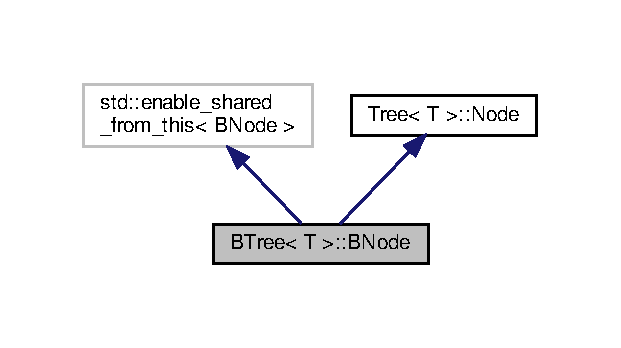
\includegraphics[width=298pt]{classBTree_1_1BNode__inherit__graph}
\end{center}
\end{figure}


Collaboration diagram for B\+Tree$<$ T $>$\+:\+:B\+Node\+:
\nopagebreak
\begin{figure}[H]
\begin{center}
\leavevmode
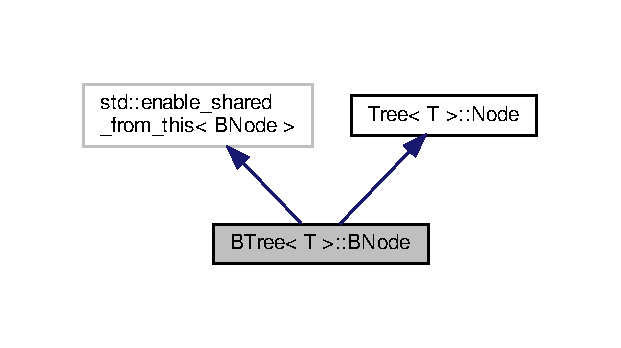
\includegraphics[width=298pt]{classBTree_1_1BNode__coll__graph}
\end{center}
\end{figure}
\subsection*{Public Member Functions}
\begin{DoxyCompactItemize}
\item 
\mbox{\Hypertarget{classBTree_1_1BNode_a6db3bbcf350e06109f86db08f86fc1d2}\label{classBTree_1_1BNode_a6db3bbcf350e06109f86db08f86fc1d2}} 
{\bfseries B\+Node} (bool is\+\_\+leaf, int min\+\_\+degree)
\item 
\mbox{\Hypertarget{classBTree_1_1BNode_a8440e89eab5284dc118c00de4e7e619b}\label{classBTree_1_1BNode_a8440e89eab5284dc118c00de4e7e619b}} 
std\+::shared\+\_\+ptr$<$ typename \hyperlink{classTree}{Tree}$<$ T $>$\+::\hyperlink{classTree_1_1Node}{Node} $>$ {\bfseries next} () noexcept override
\item 
\mbox{\Hypertarget{classBTree_1_1BNode_aa3909dab0e45cf56b602705b8720e7c0}\label{classBTree_1_1BNode_aa3909dab0e45cf56b602705b8720e7c0}} 
std\+::shared\+\_\+ptr$<$ typename \hyperlink{classTree}{Tree}$<$ T $>$\+::\hyperlink{classTree_1_1Node}{Node} $>$ {\bfseries previous} () noexcept override
\item 
\mbox{\Hypertarget{classBTree_1_1BNode_a8501fb870aca2959c7636bb0ca96424f}\label{classBTree_1_1BNode_a8501fb870aca2959c7636bb0ca96424f}} 
void {\bfseries print} ()
\item 
\mbox{\Hypertarget{classBTree_1_1BNode_a12209859c0d20881dc4197e9c677dfd5}\label{classBTree_1_1BNode_a12209859c0d20881dc4197e9c677dfd5}} 
void {\bfseries insert\+Non\+Full} (const T \&key)
\item 
\mbox{\Hypertarget{classBTree_1_1BNode_a0a8c168d152ef320e62c0283c4db3f26}\label{classBTree_1_1BNode_a0a8c168d152ef320e62c0283c4db3f26}} 
\hyperlink{classBIterator}{B\+Iterator}$<$ T $>$ {\bfseries find\+Iterator} (const T \&key)
\item 
\mbox{\Hypertarget{classBTree_1_1BNode_a559e979d22e13c7b455fef771af47049}\label{classBTree_1_1BNode_a559e979d22e13c7b455fef771af47049}} 
int {\bfseries get\+Parent\+Index} ()
\item 
\mbox{\Hypertarget{classBTree_1_1BNode_a646808ce526bbf4b5e5df0348fcca8db}\label{classBTree_1_1BNode_a646808ce526bbf4b5e5df0348fcca8db}} 
std\+::shared\+\_\+ptr$<$ \hyperlink{classBTree_1_1BNode}{B\+Node} $>$ {\bfseries find} (T key)
\item 
\mbox{\Hypertarget{classBTree_1_1BNode_a53972c6065afd789a1fdb79fe96d25e9}\label{classBTree_1_1BNode_a53972c6065afd789a1fdb79fe96d25e9}} 
int {\bfseries find\+Key} (T key)
\item 
\mbox{\Hypertarget{classBTree_1_1BNode_a2e926c4518aecdbb1dcf853431edfb0c}\label{classBTree_1_1BNode_a2e926c4518aecdbb1dcf853431edfb0c}} 
void {\bfseries remove} (T key)
\item 
\mbox{\Hypertarget{classBTree_1_1BNode_a1153066a0735afbd355c762795b68222}\label{classBTree_1_1BNode_a1153066a0735afbd355c762795b68222}} 
void {\bfseries remove\+From\+Leaf} (int idx)
\item 
\mbox{\Hypertarget{classBTree_1_1BNode_acea1502de0852161a72a4c11e122e58e}\label{classBTree_1_1BNode_acea1502de0852161a72a4c11e122e58e}} 
void {\bfseries remove\+From\+Non\+Leaf} (int idx)
\item 
\mbox{\Hypertarget{classBTree_1_1BNode_afacc18e039955c714241d33341649656}\label{classBTree_1_1BNode_afacc18e039955c714241d33341649656}} 
T {\bfseries get\+Pred} (int idx)
\item 
\mbox{\Hypertarget{classBTree_1_1BNode_af5d36fa614e035a65758f716f5902d82}\label{classBTree_1_1BNode_af5d36fa614e035a65758f716f5902d82}} 
T {\bfseries get\+Succ} (int idx)
\item 
\mbox{\Hypertarget{classBTree_1_1BNode_a20d3152742afa0fbb11e413a0c73ceb9}\label{classBTree_1_1BNode_a20d3152742afa0fbb11e413a0c73ceb9}} 
void {\bfseries fill} (int idx)
\item 
\mbox{\Hypertarget{classBTree_1_1BNode_a1ee99a5c0649e19e8a34934ff8dba85b}\label{classBTree_1_1BNode_a1ee99a5c0649e19e8a34934ff8dba85b}} 
void {\bfseries borrow\+From\+Prev} (int idx)
\item 
\mbox{\Hypertarget{classBTree_1_1BNode_acda705e13267fdedbfd27f017668a9bf}\label{classBTree_1_1BNode_acda705e13267fdedbfd27f017668a9bf}} 
void {\bfseries borrow\+From\+Next} (int idx)
\item 
\mbox{\Hypertarget{classBTree_1_1BNode_ac3caae8aac87f7bdce9960a658f9ad87}\label{classBTree_1_1BNode_ac3caae8aac87f7bdce9960a658f9ad87}} 
void {\bfseries merge} (int idx)
\item 
\mbox{\Hypertarget{classBTree_1_1BNode_a0b356b6ac1ec3d8e0cbfb68d9e5f7582}\label{classBTree_1_1BNode_a0b356b6ac1ec3d8e0cbfb68d9e5f7582}} 
void {\bfseries split\+Child} (int index, std\+::shared\+\_\+ptr$<$ \hyperlink{classBTree_1_1BNode}{B\+Node} $>$ child)
\end{DoxyCompactItemize}
\subsection*{Public Attributes}
\begin{DoxyCompactItemize}
\item 
\mbox{\Hypertarget{classBTree_1_1BNode_a5fb27046a502d2a28fc539042a1bfd87}\label{classBTree_1_1BNode_a5fb27046a502d2a28fc539042a1bfd87}} 
std\+::vector$<$ T $>$ {\bfseries keys}
\item 
\mbox{\Hypertarget{classBTree_1_1BNode_a3683e8ef7010edede627bdacb9d40025}\label{classBTree_1_1BNode_a3683e8ef7010edede627bdacb9d40025}} 
std\+::vector$<$ std\+::shared\+\_\+ptr$<$ \hyperlink{classBTree_1_1BNode}{B\+Node} $>$ $>$ {\bfseries children}
\item 
\mbox{\Hypertarget{classBTree_1_1BNode_aeea14a23dfc45f162ecbbc736b24014a}\label{classBTree_1_1BNode_aeea14a23dfc45f162ecbbc736b24014a}} 
bool {\bfseries is\+\_\+leaf}
\item 
\mbox{\Hypertarget{classBTree_1_1BNode_a9a108839cbc75c2c207d97140577bd7c}\label{classBTree_1_1BNode_a9a108839cbc75c2c207d97140577bd7c}} 
int {\bfseries min\+\_\+degree}
\item 
\mbox{\Hypertarget{classBTree_1_1BNode_a9b057ee85c9a950709afaee727515fab}\label{classBTree_1_1BNode_a9b057ee85c9a950709afaee727515fab}} 
int {\bfseries index}
\item 
\mbox{\Hypertarget{classBTree_1_1BNode_a5856f1fc1eb5e7e936d4deb50dc64a3c}\label{classBTree_1_1BNode_a5856f1fc1eb5e7e936d4deb50dc64a3c}} 
std\+::shared\+\_\+ptr$<$ \hyperlink{classBTree_1_1BNode}{B\+Node} $>$ {\bfseries parent}
\end{DoxyCompactItemize}


The documentation for this class was generated from the following file\+:\begin{DoxyCompactItemize}
\item 
src/B\+Tree.\+h\end{DoxyCompactItemize}

\hypertarget{classBplusTree_1_1BplusNode}{}\section{Bplus\+Tree$<$ T $>$\+:\+:Bplus\+Node Class Reference}
\label{classBplusTree_1_1BplusNode}\index{Bplus\+Tree$<$ T $>$\+::\+Bplus\+Node@{Bplus\+Tree$<$ T $>$\+::\+Bplus\+Node}}


Inheritance diagram for Bplus\+Tree$<$ T $>$\+:\+:Bplus\+Node\+:
\nopagebreak
\begin{figure}[H]
\begin{center}
\leavevmode
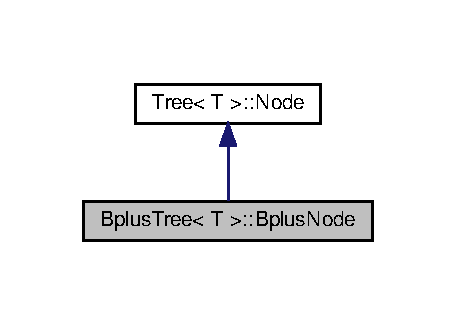
\includegraphics[width=219pt]{classBplusTree_1_1BplusNode__inherit__graph}
\end{center}
\end{figure}


Collaboration diagram for Bplus\+Tree$<$ T $>$\+:\+:Bplus\+Node\+:
\nopagebreak
\begin{figure}[H]
\begin{center}
\leavevmode
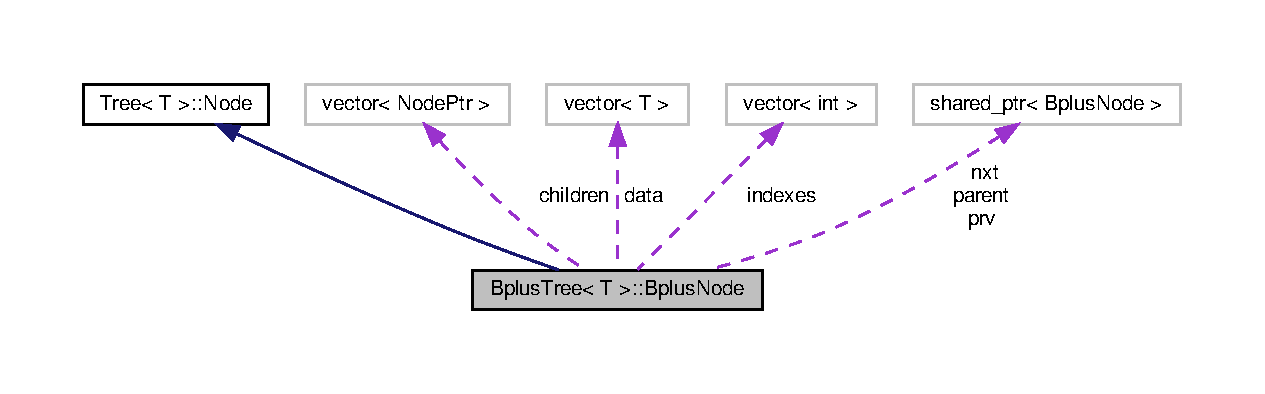
\includegraphics[width=350pt]{classBplusTree_1_1BplusNode__coll__graph}
\end{center}
\end{figure}
\subsection*{Public Member Functions}
\begin{DoxyCompactItemize}
\item 
\mbox{\Hypertarget{classBplusTree_1_1BplusNode_aa533f1a1ccceeccc83fe966d51611877}\label{classBplusTree_1_1BplusNode_aa533f1a1ccceeccc83fe966d51611877}} 
bool {\bfseries is\+\_\+leaf} () const noexcept
\item 
\mbox{\Hypertarget{classBplusTree_1_1BplusNode_ae5fa7de69c0ca98b025b0de31193d045}\label{classBplusTree_1_1BplusNode_ae5fa7de69c0ca98b025b0de31193d045}} 
std\+::shared\+\_\+ptr$<$ \hyperlink{classTree_1_1Node}{Node} $>$ {\bfseries next} () const noexcept override
\item 
\mbox{\Hypertarget{classBplusTree_1_1BplusNode_ae232d00a45a87dd854b5e6fd65ef20f9}\label{classBplusTree_1_1BplusNode_ae232d00a45a87dd854b5e6fd65ef20f9}} 
std\+::shared\+\_\+ptr$<$ \hyperlink{classTree_1_1Node}{Node} $>$ {\bfseries previous} () const noexcept override
\item 
\mbox{\Hypertarget{classBplusTree_1_1BplusNode_aef1ab31368c0247ddceb381bfd4ac144}\label{classBplusTree_1_1BplusNode_aef1ab31368c0247ddceb381bfd4ac144}} 
Node\+Ptr {\bfseries left} () const noexcept
\item 
\mbox{\Hypertarget{classBplusTree_1_1BplusNode_aa36a1f5e2c7a911603f7abbb0159bdaf}\label{classBplusTree_1_1BplusNode_aa36a1f5e2c7a911603f7abbb0159bdaf}} 
Node\+Ptr {\bfseries right} () const noexcept
\item 
\mbox{\Hypertarget{classBplusTree_1_1BplusNode_aaf30bb552543a89d3041a7248fba37db}\label{classBplusTree_1_1BplusNode_aaf30bb552543a89d3041a7248fba37db}} 
{\footnotesize template$<$typename O\+Stream $>$ }\\void {\bfseries print} (O\+Stream \&os, int level=1) const noexcept
\end{DoxyCompactItemize}
\subsection*{Public Attributes}
\begin{DoxyCompactItemize}
\item 
\mbox{\Hypertarget{classBplusTree_1_1BplusNode_a9f4cabef276864d922352ea921581edb}\label{classBplusTree_1_1BplusNode_a9f4cabef276864d922352ea921581edb}} 
Node\+Ptr {\bfseries parent}
\item 
\mbox{\Hypertarget{classBplusTree_1_1BplusNode_afd53466ca4f36766ba3c0ba96a6f7c6c}\label{classBplusTree_1_1BplusNode_afd53466ca4f36766ba3c0ba96a6f7c6c}} 
Node\+Ptr {\bfseries nxt}
\item 
\mbox{\Hypertarget{classBplusTree_1_1BplusNode_ae17e7b3bc8fa2fe184dcc564f1569b65}\label{classBplusTree_1_1BplusNode_ae17e7b3bc8fa2fe184dcc564f1569b65}} 
Node\+Ptr {\bfseries prv}
\item 
\mbox{\Hypertarget{classBplusTree_1_1BplusNode_ae602b66322e25fd68b3b75745a2a17f1}\label{classBplusTree_1_1BplusNode_ae602b66322e25fd68b3b75745a2a17f1}} 
vector$<$ Node\+Ptr $>$ {\bfseries children}
\item 
\mbox{\Hypertarget{classBplusTree_1_1BplusNode_a6b60fb47981a9aafcad811aa12502e28}\label{classBplusTree_1_1BplusNode_a6b60fb47981a9aafcad811aa12502e28}} 
vector$<$ int $>$ {\bfseries indexes}
\item 
\mbox{\Hypertarget{classBplusTree_1_1BplusNode_a889068a8a0daa157e7beed089b259df7}\label{classBplusTree_1_1BplusNode_a889068a8a0daa157e7beed089b259df7}} 
vector$<$ T $>$ {\bfseries data}
\end{DoxyCompactItemize}


The documentation for this class was generated from the following file\+:\begin{DoxyCompactItemize}
\item 
src/Bplus\+Tree.\+h\end{DoxyCompactItemize}

\hypertarget{classBplusTree}{}\section{Bplus\+Tree$<$ T $>$ Class Template Reference}
\label{classBplusTree}\index{Bplus\+Tree$<$ T $>$@{Bplus\+Tree$<$ T $>$}}


Class for implementing Bplus \hyperlink{classTree}{Tree}.  




{\ttfamily \#include $<$Bplus\+Tree.\+h$>$}



Inheritance diagram for Bplus\+Tree$<$ T $>$\+:
\nopagebreak
\begin{figure}[H]
\begin{center}
\leavevmode
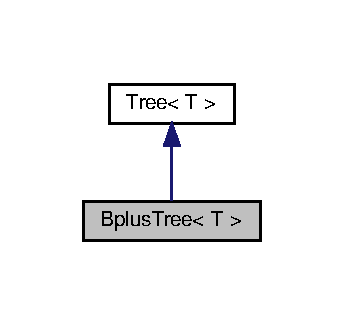
\includegraphics[width=165pt]{classBplusTree__inherit__graph}
\end{center}
\end{figure}


Collaboration diagram for Bplus\+Tree$<$ T $>$\+:
\nopagebreak
\begin{figure}[H]
\begin{center}
\leavevmode
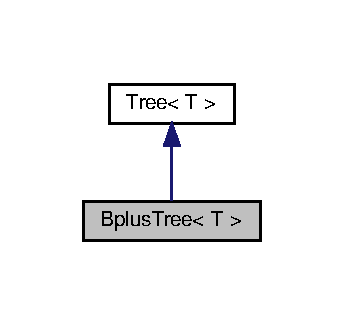
\includegraphics[width=165pt]{classBplusTree__coll__graph}
\end{center}
\end{figure}
\subsection*{Classes}
\begin{DoxyCompactItemize}
\item 
class \hyperlink{classBplusTree_1_1BplusNode}{Bplus\+Node}
\end{DoxyCompactItemize}
\subsection*{Public Types}
\begin{DoxyCompactItemize}
\item 
\mbox{\Hypertarget{classBplusTree_a4db76354142996b6c2e943e4bfe82c38}\label{classBplusTree_a4db76354142996b6c2e943e4bfe82c38}} 
typedef shared\+\_\+ptr$<$ \hyperlink{classBplusTree_1_1BplusNode}{Bplus\+Node} $>$ {\bfseries Node\+Ptr}
\end{DoxyCompactItemize}
\subsection*{Public Member Functions}
\begin{DoxyCompactItemize}
\item 
\mbox{\Hypertarget{classBplusTree_a95dac42b6d93b4c41bfcd1aacac936d8}\label{classBplusTree_a95dac42b6d93b4c41bfcd1aacac936d8}} 
{\bfseries Bplus\+Tree} (const int m)
\item 
\mbox{\Hypertarget{classBplusTree_a706e3329120bd4f25ca0e9ff28eb7e32}\label{classBplusTree_a706e3329120bd4f25ca0e9ff28eb7e32}} 
void {\bfseries insert} (const T \&key) override
\item 
\mbox{\Hypertarget{classBplusTree_a7e63275f3226fe9bdb29a4bcbd938fb4}\label{classBplusTree_a7e63275f3226fe9bdb29a4bcbd938fb4}} 
void {\bfseries remove} (const T \&key) noexcept override
\item 
\mbox{\Hypertarget{classBplusTree_ad1ae39510e9c7be66119d9387dfe30c5}\label{classBplusTree_ad1ae39510e9c7be66119d9387dfe30c5}} 
void {\bfseries print} () const noexcept override
\item 
\mbox{\Hypertarget{classBplusTree_a367ff479947c9103abc781db035a49ee}\label{classBplusTree_a367ff479947c9103abc781db035a49ee}} 
\hyperlink{classBplusIterator}{Bplus\+Iterator}$<$ T $>$ {\bfseries find} (const T \&key) const noexcept
\item 
\mbox{\Hypertarget{classBplusTree_af25d2c310a013718a1d54e8993bf7b76}\label{classBplusTree_af25d2c310a013718a1d54e8993bf7b76}} 
\hyperlink{classBplusIterator}{Bplus\+Iterator}$<$ T $>$ {\bfseries begin} () const noexcept
\item 
\mbox{\Hypertarget{classBplusTree_ac217ed576ff9495e2fd90f5d13f34065}\label{classBplusTree_ac217ed576ff9495e2fd90f5d13f34065}} 
\hyperlink{classBplusIterator}{Bplus\+Iterator}$<$ T $>$ {\bfseries end} () const noexcept
\item 
\mbox{\Hypertarget{classBplusTree_a96798aee453828de98c3eba8a6507915}\label{classBplusTree_a96798aee453828de98c3eba8a6507915}} 
\hyperlink{classBplusIterator}{Bplus\+Iterator}$<$ T $>$ {\bfseries rbegin} () const noexcept
\item 
\mbox{\Hypertarget{classBplusTree_a048e70503ad677508b75cb845d125b93}\label{classBplusTree_a048e70503ad677508b75cb845d125b93}} 
\hyperlink{classBplusIterator}{Bplus\+Iterator}$<$ T $>$ {\bfseries rend} () const noexcept
\end{DoxyCompactItemize}
\subsection*{Additional Inherited Members}


\subsection{Detailed Description}
\subsubsection*{template$<$typename T$>$\newline
class Bplus\+Tree$<$ T $>$}

Class for implementing Bplus \hyperlink{classTree}{Tree}. 

The documentation for this class was generated from the following files\+:\begin{DoxyCompactItemize}
\item 
src/Bplus\+Iterator.\+hpp\item 
src/Bplus\+Tree.\+h\end{DoxyCompactItemize}

\hypertarget{classBTree}{}\section{B\+Tree$<$ T $>$ Class Template Reference}
\label{classBTree}\index{B\+Tree$<$ T $>$@{B\+Tree$<$ T $>$}}


Class for implementing B \hyperlink{classTree}{Tree}.  




{\ttfamily \#include $<$B\+Tree.\+h$>$}



Inheritance diagram for B\+Tree$<$ T $>$\+:
\nopagebreak
\begin{figure}[H]
\begin{center}
\leavevmode
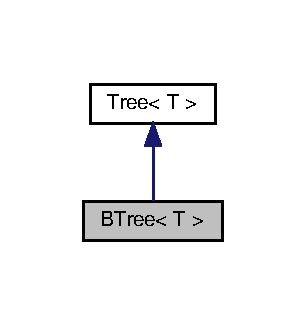
\includegraphics[width=147pt]{classBTree__inherit__graph}
\end{center}
\end{figure}


Collaboration diagram for B\+Tree$<$ T $>$\+:
\nopagebreak
\begin{figure}[H]
\begin{center}
\leavevmode
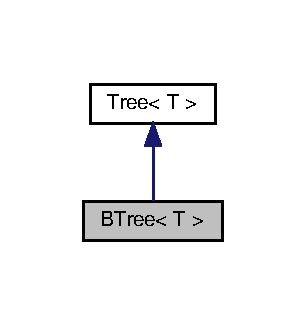
\includegraphics[width=147pt]{classBTree__coll__graph}
\end{center}
\end{figure}
\subsection*{Classes}
\begin{DoxyCompactItemize}
\item 
class \hyperlink{classBTree_1_1BNode}{B\+Node}
\end{DoxyCompactItemize}
\subsection*{Public Member Functions}
\begin{DoxyCompactItemize}
\item 
\mbox{\Hypertarget{classBTree_a16c152bc0c234a02359d259c5dd1d959}\label{classBTree_a16c152bc0c234a02359d259c5dd1d959}} 
{\bfseries B\+Tree} (int min\+\_\+degree)
\item 
\mbox{\Hypertarget{classBTree_a6b821651c388e302d1fb43551bb67232}\label{classBTree_a6b821651c388e302d1fb43551bb67232}} 
void {\bfseries insert} (const T \&key) override
\item 
\mbox{\Hypertarget{classBTree_aef3581a1c5e11ac1c037d66a27cbcb94}\label{classBTree_aef3581a1c5e11ac1c037d66a27cbcb94}} 
void {\bfseries remove} (const T \&key) noexcept override
\item 
\mbox{\Hypertarget{classBTree_a4f31693f9077aad3266b7f13625b9ede}\label{classBTree_a4f31693f9077aad3266b7f13625b9ede}} 
void {\bfseries print} () const noexcept override
\item 
\mbox{\Hypertarget{classBTree_ac0fac7271e38a543aff042db79be9c36}\label{classBTree_ac0fac7271e38a543aff042db79be9c36}} 
\hyperlink{classBIterator}{B\+Iterator}$<$ T $>$ {\bfseries find} (const T \&key) const noexcept
\item 
\mbox{\Hypertarget{classBTree_aae48f3719f14f2170641cf204a9d531c}\label{classBTree_aae48f3719f14f2170641cf204a9d531c}} 
\hyperlink{classBIterator}{B\+Iterator}$<$ T $>$ {\bfseries begin} () const noexcept
\item 
\mbox{\Hypertarget{classBTree_a3115f4378da1a0fd49e73a5dbecf9822}\label{classBTree_a3115f4378da1a0fd49e73a5dbecf9822}} 
\hyperlink{classBIterator}{B\+Iterator}$<$ T $>$ {\bfseries end} () const noexcept
\item 
\mbox{\Hypertarget{classBTree_a3a24bc55b80013d9fcd57d5589aad413}\label{classBTree_a3a24bc55b80013d9fcd57d5589aad413}} 
\hyperlink{classBIterator}{B\+Iterator}$<$ T $>$ {\bfseries rbegin} () const noexcept
\item 
\mbox{\Hypertarget{classBTree_af024f4b5201a49115da494161d4dcbce}\label{classBTree_af024f4b5201a49115da494161d4dcbce}} 
\hyperlink{classBIterator}{B\+Iterator}$<$ T $>$ {\bfseries rend} () const noexcept
\end{DoxyCompactItemize}
\subsection*{Public Attributes}
\begin{DoxyCompactItemize}
\item 
\mbox{\Hypertarget{classBTree_a67674b9ddf809c4f518185888f0918e4}\label{classBTree_a67674b9ddf809c4f518185888f0918e4}} 
int {\bfseries min\+\_\+degree}
\end{DoxyCompactItemize}


\subsection{Detailed Description}
\subsubsection*{template$<$typename T$>$\newline
class B\+Tree$<$ T $>$}

Class for implementing B \hyperlink{classTree}{Tree}. 

The documentation for this class was generated from the following files\+:\begin{DoxyCompactItemize}
\item 
src/B\+Iterator.\+hpp\item 
src/B\+Tree.\+h\end{DoxyCompactItemize}

\hypertarget{classForwardIteration}{}\section{Forward\+Iteration$<$ T $>$ Class Template Reference}
\label{classForwardIteration}\index{Forward\+Iteration$<$ T $>$@{Forward\+Iteration$<$ T $>$}}


Inheritance diagram for Forward\+Iteration$<$ T $>$\+:
\nopagebreak
\begin{figure}[H]
\begin{center}
\leavevmode
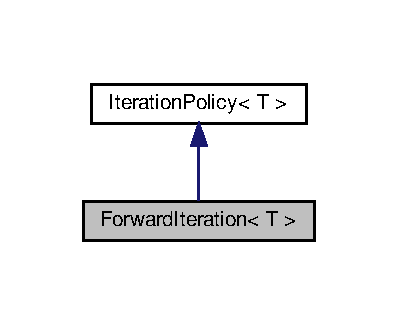
\includegraphics[width=191pt]{classForwardIteration__inherit__graph}
\end{center}
\end{figure}


Collaboration diagram for Forward\+Iteration$<$ T $>$\+:
\nopagebreak
\begin{figure}[H]
\begin{center}
\leavevmode
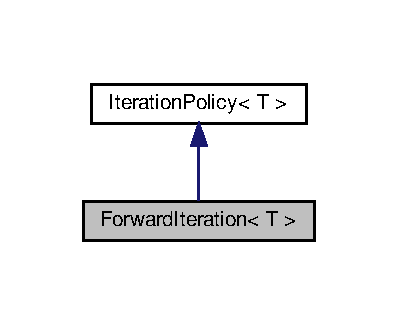
\includegraphics[width=191pt]{classForwardIteration__coll__graph}
\end{center}
\end{figure}
\subsection*{Public Member Functions}
\begin{DoxyCompactItemize}
\item 
std\+::shared\+\_\+ptr$<$ typename \hyperlink{classTree}{Tree}$<$ T $>$\+::Node $>$ \hyperlink{classForwardIteration_aec16f756354bad563a57da6157448203}{next} (std\+::shared\+\_\+ptr$<$ typename \hyperlink{classTree}{Tree}$<$ T $>$\+::Node $>$ node) const noexcept override
\begin{DoxyCompactList}\small\item\em \+: Allows us to iterate on tree in forward order \end{DoxyCompactList}\end{DoxyCompactItemize}


\subsection{Member Function Documentation}
\mbox{\Hypertarget{classForwardIteration_aec16f756354bad563a57da6157448203}\label{classForwardIteration_aec16f756354bad563a57da6157448203}} 
\index{Forward\+Iteration@{Forward\+Iteration}!next@{next}}
\index{next@{next}!Forward\+Iteration@{Forward\+Iteration}}
\subsubsection{\texorpdfstring{next()}{next()}}
{\footnotesize\ttfamily template$<$typename T $>$ \\
std\+::shared\+\_\+ptr$<$ typename \hyperlink{classTree}{Tree}$<$ T $>$\+::Node $>$ \hyperlink{classForwardIteration}{Forward\+Iteration}$<$ T $>$\+::next (\begin{DoxyParamCaption}\item[{std\+::shared\+\_\+ptr$<$ typename \hyperlink{classTree}{Tree}$<$ T $>$\+::Node $>$}]{node }\end{DoxyParamCaption}) const\hspace{0.3cm}{\ttfamily [override]}, {\ttfamily [virtual]}, {\ttfamily [noexcept]}}



\+: Allows us to iterate on tree in forward order 

Extends \hyperlink{classIterationPolicy}{Iteration\+Policy} 

Implements \hyperlink{classIterationPolicy_a69a898482a3a2ec09fd6efec002bace8}{Iteration\+Policy$<$ T $>$}.



The documentation for this class was generated from the following file\+:\begin{DoxyCompactItemize}
\item 
src/Iteration\+Policy.\+h\end{DoxyCompactItemize}

\hypertarget{classIterationPolicy}{}\section{Iteration\+Policy$<$ T $>$ Class Template Reference}
\label{classIterationPolicy}\index{Iteration\+Policy$<$ T $>$@{Iteration\+Policy$<$ T $>$}}


Inheritance diagram for Iteration\+Policy$<$ T $>$\+:\nopagebreak
\begin{figure}[H]
\begin{center}
\leavevmode
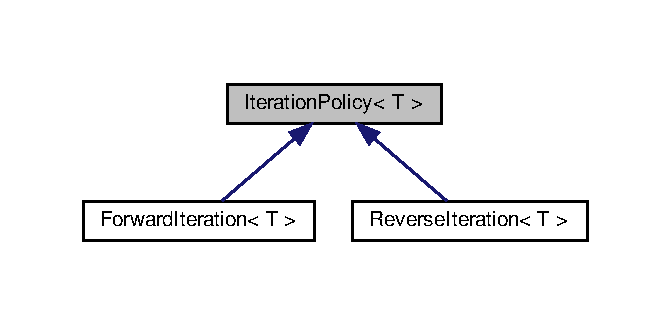
\includegraphics[width=322pt]{classIterationPolicy__inherit__graph}
\end{center}
\end{figure}
\subsection*{Public Member Functions}
\begin{DoxyCompactItemize}
\item 
virtual std\+::shared\+\_\+ptr$<$ typename \hyperlink{classTree}{Tree}$<$ T $>$\+::Node $>$ \hyperlink{classIterationPolicy_a69a898482a3a2ec09fd6efec002bace8}{next} (std\+::shared\+\_\+ptr$<$ typename \hyperlink{classTree}{Tree}$<$ T $>$\+::Node $>$ node) const noexcept=0
\begin{DoxyCompactList}\small\item\em \+: Defines behaviour of iterator using Iteration\+Policy\+::next(node) \end{DoxyCompactList}\end{DoxyCompactItemize}


\subsection{Member Function Documentation}
\mbox{\Hypertarget{classIterationPolicy_a69a898482a3a2ec09fd6efec002bace8}\label{classIterationPolicy_a69a898482a3a2ec09fd6efec002bace8}} 
\index{Iteration\+Policy@{Iteration\+Policy}!next@{next}}
\index{next@{next}!Iteration\+Policy@{Iteration\+Policy}}
\subsubsection{\texorpdfstring{next()}{next()}}
{\footnotesize\ttfamily template$<$typename T $>$ \\
virtual std\+::shared\+\_\+ptr$<$typename \hyperlink{classTree}{Tree}$<$T$>$\+::Node$>$ \hyperlink{classIterationPolicy}{Iteration\+Policy}$<$ T $>$\+::next (\begin{DoxyParamCaption}\item[{std\+::shared\+\_\+ptr$<$ typename \hyperlink{classTree}{Tree}$<$ T $>$\+::Node $>$}]{node }\end{DoxyParamCaption}) const\hspace{0.3cm}{\ttfamily [pure virtual]}, {\ttfamily [noexcept]}}



\+: Defines behaviour of iterator using Iteration\+Policy\+::next(node) 

Base class for iteration policies 

Implemented in \hyperlink{classReverseIteration_a3ca61dfcdf068fcc2905106a800c96fb}{Reverse\+Iteration$<$ T $>$}, and \hyperlink{classForwardIteration_aec16f756354bad563a57da6157448203}{Forward\+Iteration$<$ T $>$}.



The documentation for this class was generated from the following file\+:\begin{DoxyCompactItemize}
\item 
src/Iteration\+Policy.\+h\end{DoxyCompactItemize}

\hypertarget{classTree_1_1Node}{}\section{Tree$<$ T $>$\+:\+:Node Class Reference}
\label{classTree_1_1Node}\index{Tree$<$ T $>$\+::\+Node@{Tree$<$ T $>$\+::\+Node}}


Base Class for all nodes.  




{\ttfamily \#include $<$Tree.\+h$>$}



Inheritance diagram for Tree$<$ T $>$\+:\+:Node\+:
\nopagebreak
\begin{figure}[H]
\begin{center}
\leavevmode
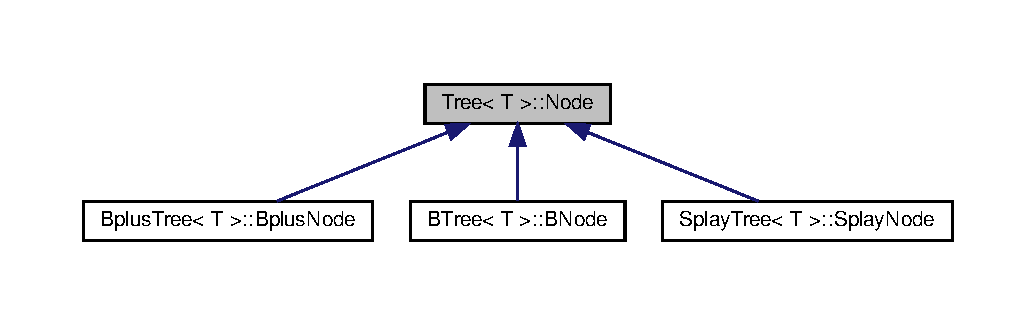
\includegraphics[width=350pt]{classTree_1_1Node__inherit__graph}
\end{center}
\end{figure}
\subsection*{Public Member Functions}
\begin{DoxyCompactItemize}
\item 
virtual std\+::shared\+\_\+ptr$<$ \hyperlink{classTree_1_1Node}{Node} $>$ \hyperlink{classTree_1_1Node_a50f15b262b0d6c572904be68ba067ca6}{next} () noexcept=0
\begin{DoxyCompactList}\small\item\em get next element ordered by keys \end{DoxyCompactList}\item 
virtual std\+::shared\+\_\+ptr$<$ \hyperlink{classTree_1_1Node}{Node} $>$ \hyperlink{classTree_1_1Node_a3f912d90adc2c50de5ce7f96e6695c96}{previous} () noexcept=0
\begin{DoxyCompactList}\small\item\em get previous element ordered by keys \end{DoxyCompactList}\end{DoxyCompactItemize}


\subsection{Detailed Description}
\subsubsection*{template$<$typename T$>$\newline
class Tree$<$ T $>$\+::\+Node}

Base Class for all nodes. 

\subsection{Member Function Documentation}
\mbox{\Hypertarget{classTree_1_1Node_a50f15b262b0d6c572904be68ba067ca6}\label{classTree_1_1Node_a50f15b262b0d6c572904be68ba067ca6}} 
\index{Tree\+::\+Node@{Tree\+::\+Node}!next@{next}}
\index{next@{next}!Tree\+::\+Node@{Tree\+::\+Node}}
\subsubsection{\texorpdfstring{next()}{next()}}
{\footnotesize\ttfamily template$<$typename T $>$ \\
virtual std\+::shared\+\_\+ptr$<$\hyperlink{classTree_1_1Node}{Node}$>$ \hyperlink{classTree}{Tree}$<$ T $>$\+::Node\+::next (\begin{DoxyParamCaption}{ }\end{DoxyParamCaption})\hspace{0.3cm}{\ttfamily [pure virtual]}, {\ttfamily [noexcept]}}



get next element ordered by keys 

\begin{DoxyReturn}{Returns}
nullptr if not exist 
\end{DoxyReturn}


Implemented in \hyperlink{classBTree_1_1BNode_a8440e89eab5284dc118c00de4e7e619b}{B\+Tree$<$ T $>$\+::\+B\+Node}, and \hyperlink{classSplayTree_1_1SplayNode_a958decc1fc4c1c2aa4c80c5fc4e42acd}{Splay\+Tree$<$ T $>$\+::\+Splay\+Node}.

\mbox{\Hypertarget{classTree_1_1Node_a3f912d90adc2c50de5ce7f96e6695c96}\label{classTree_1_1Node_a3f912d90adc2c50de5ce7f96e6695c96}} 
\index{Tree\+::\+Node@{Tree\+::\+Node}!previous@{previous}}
\index{previous@{previous}!Tree\+::\+Node@{Tree\+::\+Node}}
\subsubsection{\texorpdfstring{previous()}{previous()}}
{\footnotesize\ttfamily template$<$typename T $>$ \\
virtual std\+::shared\+\_\+ptr$<$\hyperlink{classTree_1_1Node}{Node}$>$ \hyperlink{classTree}{Tree}$<$ T $>$\+::Node\+::previous (\begin{DoxyParamCaption}{ }\end{DoxyParamCaption})\hspace{0.3cm}{\ttfamily [pure virtual]}, {\ttfamily [noexcept]}}



get previous element ordered by keys 

\begin{DoxyReturn}{Returns}
nullptr if not exist 
\end{DoxyReturn}


Implemented in \hyperlink{classBTree_1_1BNode_aa3909dab0e45cf56b602705b8720e7c0}{B\+Tree$<$ T $>$\+::\+B\+Node}, and \hyperlink{classSplayTree_1_1SplayNode_a6a89136b18f560485a4bda43ef15f560}{Splay\+Tree$<$ T $>$\+::\+Splay\+Node}.



The documentation for this class was generated from the following file\+:\begin{DoxyCompactItemize}
\item 
src/Tree.\+h\end{DoxyCompactItemize}

\hypertarget{classReverseIteration}{}\section{Reverse\+Iteration$<$ T $>$ Class Template Reference}
\label{classReverseIteration}\index{Reverse\+Iteration$<$ T $>$@{Reverse\+Iteration$<$ T $>$}}


Inheritance diagram for Reverse\+Iteration$<$ T $>$\+:\nopagebreak
\begin{figure}[H]
\begin{center}
\leavevmode
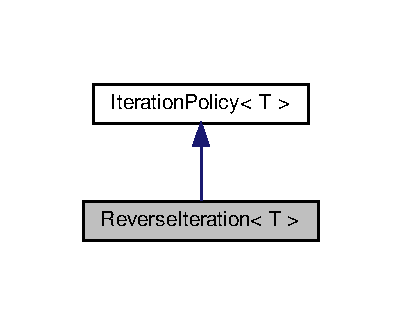
\includegraphics[width=193pt]{classReverseIteration__inherit__graph}
\end{center}
\end{figure}


Collaboration diagram for Reverse\+Iteration$<$ T $>$\+:\nopagebreak
\begin{figure}[H]
\begin{center}
\leavevmode
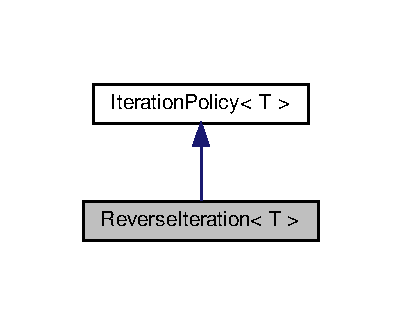
\includegraphics[width=193pt]{classReverseIteration__coll__graph}
\end{center}
\end{figure}
\subsection*{Public Member Functions}
\begin{DoxyCompactItemize}
\item 
std\+::shared\+\_\+ptr$<$ typename \hyperlink{classTree}{Tree}$<$ T $>$\+::Node $>$ \hyperlink{classReverseIteration_a3ca61dfcdf068fcc2905106a800c96fb}{next} (std\+::shared\+\_\+ptr$<$ typename \hyperlink{classTree}{Tree}$<$ T $>$\+::Node $>$ node) const noexcept override
\begin{DoxyCompactList}\small\item\em \+: Allows us to iterate on tree in reverse order \end{DoxyCompactList}\end{DoxyCompactItemize}


\subsection{Member Function Documentation}
\mbox{\Hypertarget{classReverseIteration_a3ca61dfcdf068fcc2905106a800c96fb}\label{classReverseIteration_a3ca61dfcdf068fcc2905106a800c96fb}} 
\index{Reverse\+Iteration@{Reverse\+Iteration}!next@{next}}
\index{next@{next}!Reverse\+Iteration@{Reverse\+Iteration}}
\subsubsection{\texorpdfstring{next()}{next()}}
{\footnotesize\ttfamily template$<$typename T $>$ \\
std\+::shared\+\_\+ptr$<$ typename \hyperlink{classTree}{Tree}$<$ T $>$\+::Node $>$ \hyperlink{classReverseIteration}{Reverse\+Iteration}$<$ T $>$\+::next (\begin{DoxyParamCaption}\item[{std\+::shared\+\_\+ptr$<$ typename \hyperlink{classTree}{Tree}$<$ T $>$\+::Node $>$}]{node }\end{DoxyParamCaption}) const\hspace{0.3cm}{\ttfamily [override]}, {\ttfamily [virtual]}, {\ttfamily [noexcept]}}



\+: Allows us to iterate on tree in reverse order 

Extends \hyperlink{classIterationPolicy}{Iteration\+Policy} 

Implements \hyperlink{classIterationPolicy_a69a898482a3a2ec09fd6efec002bace8}{Iteration\+Policy$<$ T $>$}.



The documentation for this class was generated from the following file\+:\begin{DoxyCompactItemize}
\item 
src/Iteration\+Policy.\+h\end{DoxyCompactItemize}

\hypertarget{classSplayIterator}{}\section{Splay\+Iterator$<$ T $>$ Class Template Reference}
\label{classSplayIterator}\index{Splay\+Iterator$<$ T $>$@{Splay\+Iterator$<$ T $>$}}
\subsection*{Public Member Functions}
\begin{DoxyCompactItemize}
\item 
\mbox{\Hypertarget{classSplayIterator_a41a5dce71eee4a8b82025efe547ae1aa}\label{classSplayIterator_a41a5dce71eee4a8b82025efe547ae1aa}} 
{\bfseries Splay\+Iterator} (std\+::shared\+\_\+ptr$<$ typename \hyperlink{classSplayTree}{Splay\+Tree}$<$ T $>$\+::Splay\+Node $>$ root, std\+::shared\+\_\+ptr$<$ \hyperlink{classIterationPolicy}{Iteration\+Policy}$<$ T $>$$>$ policy)
\item 
\mbox{\Hypertarget{classSplayIterator_ab25826d70fa08b45174d7006b1c7f43e}\label{classSplayIterator_ab25826d70fa08b45174d7006b1c7f43e}} 
virtual const T \& {\bfseries operator$\ast$} () const noexcept
\item 
\mbox{\Hypertarget{classSplayIterator_a7fd3ee4bfaac3622600cdf85f4752327}\label{classSplayIterator_a7fd3ee4bfaac3622600cdf85f4752327}} 
virtual bool {\bfseries operator!=} (const \hyperlink{classSplayIterator}{Splay\+Iterator} \&other) noexcept
\item 
\mbox{\Hypertarget{classSplayIterator_aa346bf707e077d808dfc3a0cc090ad69}\label{classSplayIterator_aa346bf707e077d808dfc3a0cc090ad69}} 
virtual bool {\bfseries operator==} (const \hyperlink{classSplayIterator}{Splay\+Iterator} \&other) noexcept
\item 
\mbox{\Hypertarget{classSplayIterator_a5493e9ce13e85ac77ed47fef6fafdb0e}\label{classSplayIterator_a5493e9ce13e85ac77ed47fef6fafdb0e}} 
\hyperlink{classSplayIterator}{Splay\+Iterator} \& {\bfseries operator++} () noexcept
\item 
\mbox{\Hypertarget{classSplayIterator_a9566d71720c54a8c1ac4edc0117413d0}\label{classSplayIterator_a9566d71720c54a8c1ac4edc0117413d0}} 
\hyperlink{classSplayIterator}{Splay\+Iterator} {\bfseries operator+} (int n) const noexcept
\end{DoxyCompactItemize}
\subsection*{Protected Attributes}
\begin{DoxyCompactItemize}
\item 
\mbox{\Hypertarget{classSplayIterator_a3a6e76a1cce8cb5127c68de23bbde2b6}\label{classSplayIterator_a3a6e76a1cce8cb5127c68de23bbde2b6}} 
std\+::shared\+\_\+ptr$<$ typename \hyperlink{classSplayTree}{Splay\+Tree}$<$ T $>$\+::Splay\+Node $>$ {\bfseries curr\+\_\+node}
\item 
\mbox{\Hypertarget{classSplayIterator_ada3c3096d608ed5e8bed651c1b9f8df6}\label{classSplayIterator_ada3c3096d608ed5e8bed651c1b9f8df6}} 
std\+::shared\+\_\+ptr$<$ \hyperlink{classIterationPolicy}{Iteration\+Policy}$<$ T $>$ $>$ {\bfseries policy}
\end{DoxyCompactItemize}
\subsection*{Friends}
\begin{DoxyCompactItemize}
\item 
class \hyperlink{classSplayIterator_a151ca71f2c751d8a163f3f99ccf6cec9}{Tree$<$ T $>$}
\begin{DoxyCompactList}\small\item\em \+: Allows us to write specific iterators for trees, and define iterating behaviour with \hyperlink{classIterationPolicy}{Iteration\+Policy} (Mix of Bridge and Strategy Patterns) \end{DoxyCompactList}\end{DoxyCompactItemize}


\subsection{Friends And Related Function Documentation}
\mbox{\Hypertarget{classSplayIterator_a151ca71f2c751d8a163f3f99ccf6cec9}\label{classSplayIterator_a151ca71f2c751d8a163f3f99ccf6cec9}} 
\index{Splay\+Iterator@{Splay\+Iterator}!Tree$<$ T $>$@{Tree$<$ T $>$}}
\index{Tree$<$ T $>$@{Tree$<$ T $>$}!Splay\+Iterator@{Splay\+Iterator}}
\subsubsection{\texorpdfstring{Tree$<$ T $>$}{Tree< T >}}
{\footnotesize\ttfamily template$<$typename T $>$ \\
friend class \hyperlink{classTree}{Tree}$<$ T $>$\hspace{0.3cm}{\ttfamily [friend]}}



\+: Allows us to write specific iterators for trees, and define iterating behaviour with \hyperlink{classIterationPolicy}{Iteration\+Policy} (Mix of Bridge and Strategy Patterns) 

Base class-\/interface for iterators 

The documentation for this class was generated from the following file\+:\begin{DoxyCompactItemize}
\item 
src/Splay\+Iterator.\+hpp\end{DoxyCompactItemize}

\hypertarget{classSplayTree_1_1SplayNode}{}\section{Splay\+Tree$<$ T $>$\+:\+:Splay\+Node Class Reference}
\label{classSplayTree_1_1SplayNode}\index{Splay\+Tree$<$ T $>$\+::\+Splay\+Node@{Splay\+Tree$<$ T $>$\+::\+Splay\+Node}}


Inheritance diagram for Splay\+Tree$<$ T $>$\+:\+:Splay\+Node\+:
\nopagebreak
\begin{figure}[H]
\begin{center}
\leavevmode
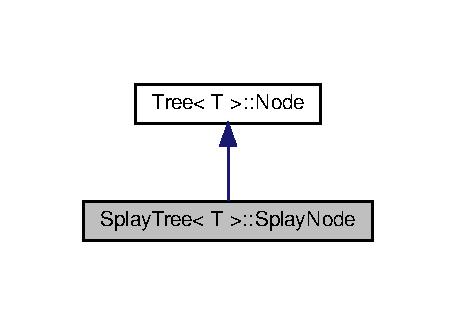
\includegraphics[width=219pt]{classSplayTree_1_1SplayNode__inherit__graph}
\end{center}
\end{figure}


Collaboration diagram for Splay\+Tree$<$ T $>$\+:\+:Splay\+Node\+:
\nopagebreak
\begin{figure}[H]
\begin{center}
\leavevmode
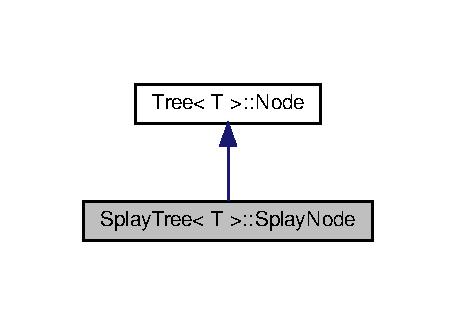
\includegraphics[width=219pt]{classSplayTree_1_1SplayNode__coll__graph}
\end{center}
\end{figure}
\subsection*{Public Member Functions}
\begin{DoxyCompactItemize}
\item 
\mbox{\Hypertarget{classSplayTree_1_1SplayNode_af613da62a8442f16ac8b4d2f1a2c9a41}\label{classSplayTree_1_1SplayNode_af613da62a8442f16ac8b4d2f1a2c9a41}} 
{\bfseries Splay\+Node} (const T \&key)
\item 
\mbox{\Hypertarget{classSplayTree_1_1SplayNode_a958decc1fc4c1c2aa4c80c5fc4e42acd}\label{classSplayTree_1_1SplayNode_a958decc1fc4c1c2aa4c80c5fc4e42acd}} 
std\+::shared\+\_\+ptr$<$ typename \hyperlink{classTree}{Tree}$<$ T $>$\+::\hyperlink{classTree_1_1Node}{Node} $>$ {\bfseries next} () noexcept override
\item 
\mbox{\Hypertarget{classSplayTree_1_1SplayNode_a6a89136b18f560485a4bda43ef15f560}\label{classSplayTree_1_1SplayNode_a6a89136b18f560485a4bda43ef15f560}} 
std\+::shared\+\_\+ptr$<$ typename \hyperlink{classTree}{Tree}$<$ T $>$\+::\hyperlink{classTree_1_1Node}{Node} $>$ {\bfseries previous} () noexcept override
\item 
\mbox{\Hypertarget{classSplayTree_1_1SplayNode_ac057d0b4f3e979f4145e4690c8edc343}\label{classSplayTree_1_1SplayNode_ac057d0b4f3e979f4145e4690c8edc343}} 
bool {\bfseries is\+Left\+Son} () const noexcept
\item 
\mbox{\Hypertarget{classSplayTree_1_1SplayNode_a650c250d2034ffea6db16daf30114ad3}\label{classSplayTree_1_1SplayNode_a650c250d2034ffea6db16daf30114ad3}} 
bool {\bfseries is\+Right\+Son} () const noexcept
\end{DoxyCompactItemize}
\subsection*{Public Attributes}
\begin{DoxyCompactItemize}
\item 
\mbox{\Hypertarget{classSplayTree_1_1SplayNode_a4c3d24b5fe0a6220132892e341c3fe34}\label{classSplayTree_1_1SplayNode_a4c3d24b5fe0a6220132892e341c3fe34}} 
T {\bfseries data}
\item 
\mbox{\Hypertarget{classSplayTree_1_1SplayNode_a8aeaae9e2fa624ee436abd87bd90eefb}\label{classSplayTree_1_1SplayNode_a8aeaae9e2fa624ee436abd87bd90eefb}} 
std\+::shared\+\_\+ptr$<$ \hyperlink{classSplayTree_1_1SplayNode}{Splay\+Node} $>$ {\bfseries parent}
\item 
\mbox{\Hypertarget{classSplayTree_1_1SplayNode_abc672e50545562d79fe247fe4959c6a0}\label{classSplayTree_1_1SplayNode_abc672e50545562d79fe247fe4959c6a0}} 
std\+::shared\+\_\+ptr$<$ \hyperlink{classSplayTree_1_1SplayNode}{Splay\+Node} $>$ {\bfseries left}
\item 
\mbox{\Hypertarget{classSplayTree_1_1SplayNode_ac72b70dd81da0a57e1e2678a4da0e0cf}\label{classSplayTree_1_1SplayNode_ac72b70dd81da0a57e1e2678a4da0e0cf}} 
std\+::shared\+\_\+ptr$<$ \hyperlink{classSplayTree_1_1SplayNode}{Splay\+Node} $>$ {\bfseries right}
\end{DoxyCompactItemize}


The documentation for this class was generated from the following file\+:\begin{DoxyCompactItemize}
\item 
src/Splay\+Tree.\+h\end{DoxyCompactItemize}

\hypertarget{classSplayTree}{}\section{Splay\+Tree$<$ T $>$ Class Template Reference}
\label{classSplayTree}\index{Splay\+Tree$<$ T $>$@{Splay\+Tree$<$ T $>$}}


Class for implementing Splay \hyperlink{classTree}{Tree}.  




{\ttfamily \#include $<$Splay\+Tree.\+h$>$}



Inheritance diagram for Splay\+Tree$<$ T $>$\+:
\nopagebreak
\begin{figure}[H]
\begin{center}
\leavevmode
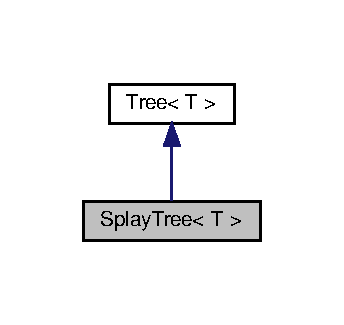
\includegraphics[width=165pt]{classSplayTree__inherit__graph}
\end{center}
\end{figure}


Collaboration diagram for Splay\+Tree$<$ T $>$\+:
\nopagebreak
\begin{figure}[H]
\begin{center}
\leavevmode
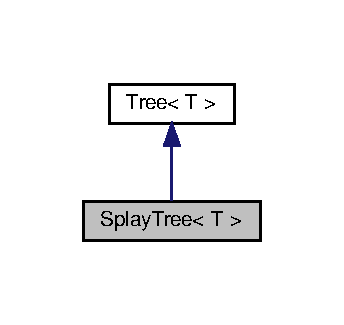
\includegraphics[width=165pt]{classSplayTree__coll__graph}
\end{center}
\end{figure}
\subsection*{Classes}
\begin{DoxyCompactItemize}
\item 
class \hyperlink{classSplayTree_1_1SplayNode}{Splay\+Node}
\end{DoxyCompactItemize}
\subsection*{Public Member Functions}
\begin{DoxyCompactItemize}
\item 
\mbox{\Hypertarget{classSplayTree_a855f0e55be8ad7d01f5b0330ee0025b0}\label{classSplayTree_a855f0e55be8ad7d01f5b0330ee0025b0}} 
void {\bfseries insert} (const T \&key) override
\item 
\mbox{\Hypertarget{classSplayTree_a5bdc3f8e97386b08e9526f4f93def2cf}\label{classSplayTree_a5bdc3f8e97386b08e9526f4f93def2cf}} 
void {\bfseries remove} (const T \&key) noexcept override
\item 
\mbox{\Hypertarget{classSplayTree_a5299790551c2576d621ebc47f47f413d}\label{classSplayTree_a5299790551c2576d621ebc47f47f413d}} 
void {\bfseries print} () const noexcept override
\item 
\mbox{\Hypertarget{classSplayTree_a97b654c8ebfb8e780dc4a46fb1e1197a}\label{classSplayTree_a97b654c8ebfb8e780dc4a46fb1e1197a}} 
\hyperlink{classSplayIterator}{Splay\+Iterator}$<$ T $>$ {\bfseries find} (const T \&key) const noexcept
\item 
\mbox{\Hypertarget{classSplayTree_afb4da5395fe3815703b7741e92b50fdd}\label{classSplayTree_afb4da5395fe3815703b7741e92b50fdd}} 
\hyperlink{classSplayIterator}{Splay\+Iterator}$<$ T $>$ {\bfseries begin} () const noexcept
\item 
\mbox{\Hypertarget{classSplayTree_a9aff68b59f341ff1a9455101836d9e44}\label{classSplayTree_a9aff68b59f341ff1a9455101836d9e44}} 
\hyperlink{classSplayIterator}{Splay\+Iterator}$<$ T $>$ {\bfseries end} () const noexcept
\item 
\mbox{\Hypertarget{classSplayTree_a073db12fe9a7269cf09c284a5960d0e0}\label{classSplayTree_a073db12fe9a7269cf09c284a5960d0e0}} 
\hyperlink{classSplayIterator}{Splay\+Iterator}$<$ T $>$ {\bfseries rbegin} () const noexcept
\item 
\mbox{\Hypertarget{classSplayTree_aeab592029a72feadab4b848ebc7e3665}\label{classSplayTree_aeab592029a72feadab4b848ebc7e3665}} 
\hyperlink{classSplayIterator}{Splay\+Iterator}$<$ T $>$ {\bfseries rend} () const noexcept
\end{DoxyCompactItemize}
\subsection*{Additional Inherited Members}


\subsection{Detailed Description}
\subsubsection*{template$<$typename T$>$\newline
class Splay\+Tree$<$ T $>$}

Class for implementing Splay \hyperlink{classTree}{Tree}. 

The documentation for this class was generated from the following files\+:\begin{DoxyCompactItemize}
\item 
src/Splay\+Iterator.\+hpp\item 
src/Splay\+Tree.\+h\end{DoxyCompactItemize}

\hypertarget{classTree}{}\section{Tree$<$ T $>$ Class Template Reference}
\label{classTree}\index{Tree$<$ T $>$@{Tree$<$ T $>$}}


Base class for all Trees  Used for making similar interface for all Trees.  




{\ttfamily \#include $<$Tree.\+h$>$}



Inheritance diagram for Tree$<$ T $>$\+:\nopagebreak
\begin{figure}[H]
\begin{center}
\leavevmode
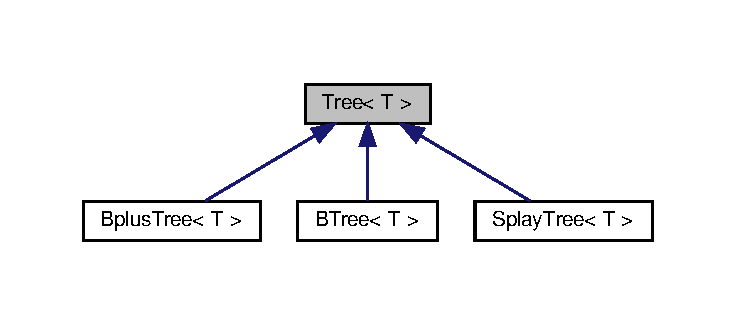
\includegraphics[width=350pt]{classTree__inherit__graph}
\end{center}
\end{figure}
\subsection*{Classes}
\begin{DoxyCompactItemize}
\item 
class \hyperlink{classTree_1_1Node}{Node}
\begin{DoxyCompactList}\small\item\em Base Class for all nodes. \end{DoxyCompactList}\end{DoxyCompactItemize}
\subsection*{Public Member Functions}
\begin{DoxyCompactItemize}
\item 
\mbox{\Hypertarget{classTree_a33de7916dcffea3a4bebe97584f1c5c1}\label{classTree_a33de7916dcffea3a4bebe97584f1c5c1}} 
virtual void \hyperlink{classTree_a33de7916dcffea3a4bebe97584f1c5c1}{insert} (const T \&key)=0
\begin{DoxyCompactList}\small\item\em Insert element in the tree with Template parameter key. \end{DoxyCompactList}\item 
\mbox{\Hypertarget{classTree_a24d087ff6f8a6f342717361825280fda}\label{classTree_a24d087ff6f8a6f342717361825280fda}} 
virtual void \hyperlink{classTree_a24d087ff6f8a6f342717361825280fda}{remove} (const T \&key) noexcept=0
\begin{DoxyCompactList}\small\item\em remove element from the tree with Template parameter key  if there is no element with this key -\/ nothing does \end{DoxyCompactList}\item 
\mbox{\Hypertarget{classTree_ae6779310befe6ae12ac32f93195bdfe3}\label{classTree_ae6779310befe6ae12ac32f93195bdfe3}} 
virtual void \hyperlink{classTree_ae6779310befe6ae12ac32f93195bdfe3}{print} () const noexcept=0
\begin{DoxyCompactList}\small\item\em simple print tree in console  can be done with Iterators \end{DoxyCompactList}\end{DoxyCompactItemize}
\subsection*{Public Attributes}
\begin{DoxyCompactItemize}
\item 
\mbox{\Hypertarget{classTree_a32eaa5ce266bb8896b57fb5527b6c8e9}\label{classTree_a32eaa5ce266bb8896b57fb5527b6c8e9}} 
std\+::shared\+\_\+ptr$<$ \hyperlink{classTree_1_1Node}{Node} $>$ {\bfseries root}
\end{DoxyCompactItemize}


\subsection{Detailed Description}
\subsubsection*{template$<$typename T$>$\newline
class Tree$<$ T $>$}

Base class for all Trees  Used for making similar interface for all Trees. 

The documentation for this class was generated from the following files\+:\begin{DoxyCompactItemize}
\item 
src/B\+Iterator.\+hpp\item 
src/Tree.\+h\end{DoxyCompactItemize}

%--- End generated contents ---

% Index
\backmatter
\newpage
\phantomsection
\clearemptydoublepage
\addcontentsline{toc}{chapter}{Index}
\printindex

\end{document}
